\documentclass[10pt]{article}
\usepackage[margin=0.85in]{geometry}
\usepackage{amsmath,amssymb,booktabs,array,tabularx,xcolor,enumitem,caption}
\usepackage{xurl}
\usepackage{hyperref}
\usepackage{tikz}
\usetikzlibrary{positioning,arrows.meta,fit,backgrounds,calc,shapes.geometric}
\hypersetup{colorlinks=true,linkcolor=blue!50!black,urlcolor=blue!50!black}
\setlist{itemsep=1pt,topsep=3pt}
\definecolor{enc}{HTML}{DCE8F7}
\definecolor{dec}{HTML}{FBE3D6}
\definecolor{lat}{HTML}{E4DDF4}
\definecolor{inp}{HTML}{EDEDEA}
\definecolor{var}{HTML}{D7F0E6}
\definecolor{ink}{HTML}{333333}
\newcommand{\code}[1]{\texttt{\small #1}}
\newcommand{\shape}[1]{{\small\ttfamily [#1]}}
\newcommand{\cp}[1]{{\small\path{#1}}}

\title{STARS multi-agent forecaster and simulator:\\ architecture, variants, inputs/outputs and losses}
\author{Code: \code{michaelmunje/stars\_steps\_extension}, branch \code{stars-rollout-ft} @ \code{5d37a3a}}
\date{2026-11-18}

\begin{document}
\maketitle

\noindent
This note describes exactly what the STARS forecaster computes, how every variant we trained differs
from it, what goes in and what comes out (with a worked example), how it is run as a closed-loop crowd
simulator, and (in the appendix) every loss term, hyperparameter, evaluation metric and the code
location of each piece. Line numbers refer to branch \code{stars-rollout-ft} at commit \code{5d37a3a},
which contains all variants; paths are relative to the repository root.

\tableofcontents

%======================================================================
\section{Notation and the forecasting task}
%======================================================================
\begin{tabular}{@{}ll@{}}
\toprule
$N$ & number of pedestrians (agents) in the scene window \\
$T=8$ & observed steps (3.2 s), $\Delta t = 0.4$ s \\
$P=12$ & predicted steps (4.8 s) \\
$K$ & number of sampled futures per scene (20 in all benchmarks) \\
$\mathbf{x}_i^{1:T}$ & observed positions of agent $i$ (scene frame, metres) \\
$\mathbf{y}_i^{1:P}$ & true future positions of agent $i$ (training targets only) \\
$m_{i,t}\in\{0,1\}$ & validity mask (agent visible at step $t$) \\
$c_i$ & per-agent decoder context; $z_i$ per-agent intent latent \\
\bottomrule
\end{tabular}

\medskip
\noindent\textbf{Task.} Given every agent's last $T$ positions in one scene, output $K$ joint futures
\shape{K, N, 12, 2}: sample $k$ assigns one 12-step future to every agent. Each agent is processed in its
own \emph{local frame}: origin at its last observed position, $x$-axis along its current heading
(\code{stars\_ma\_graph.py:105}); predictions are rotated back to the scene frame at the end
(\code{to\_scene}, \code{stars\_ma\_graph.py:201}).

%======================================================================
\section{The core model (\code{StarsMultiAgentForecaster})}
%======================================================================

\begin{figure}[p]
\centering
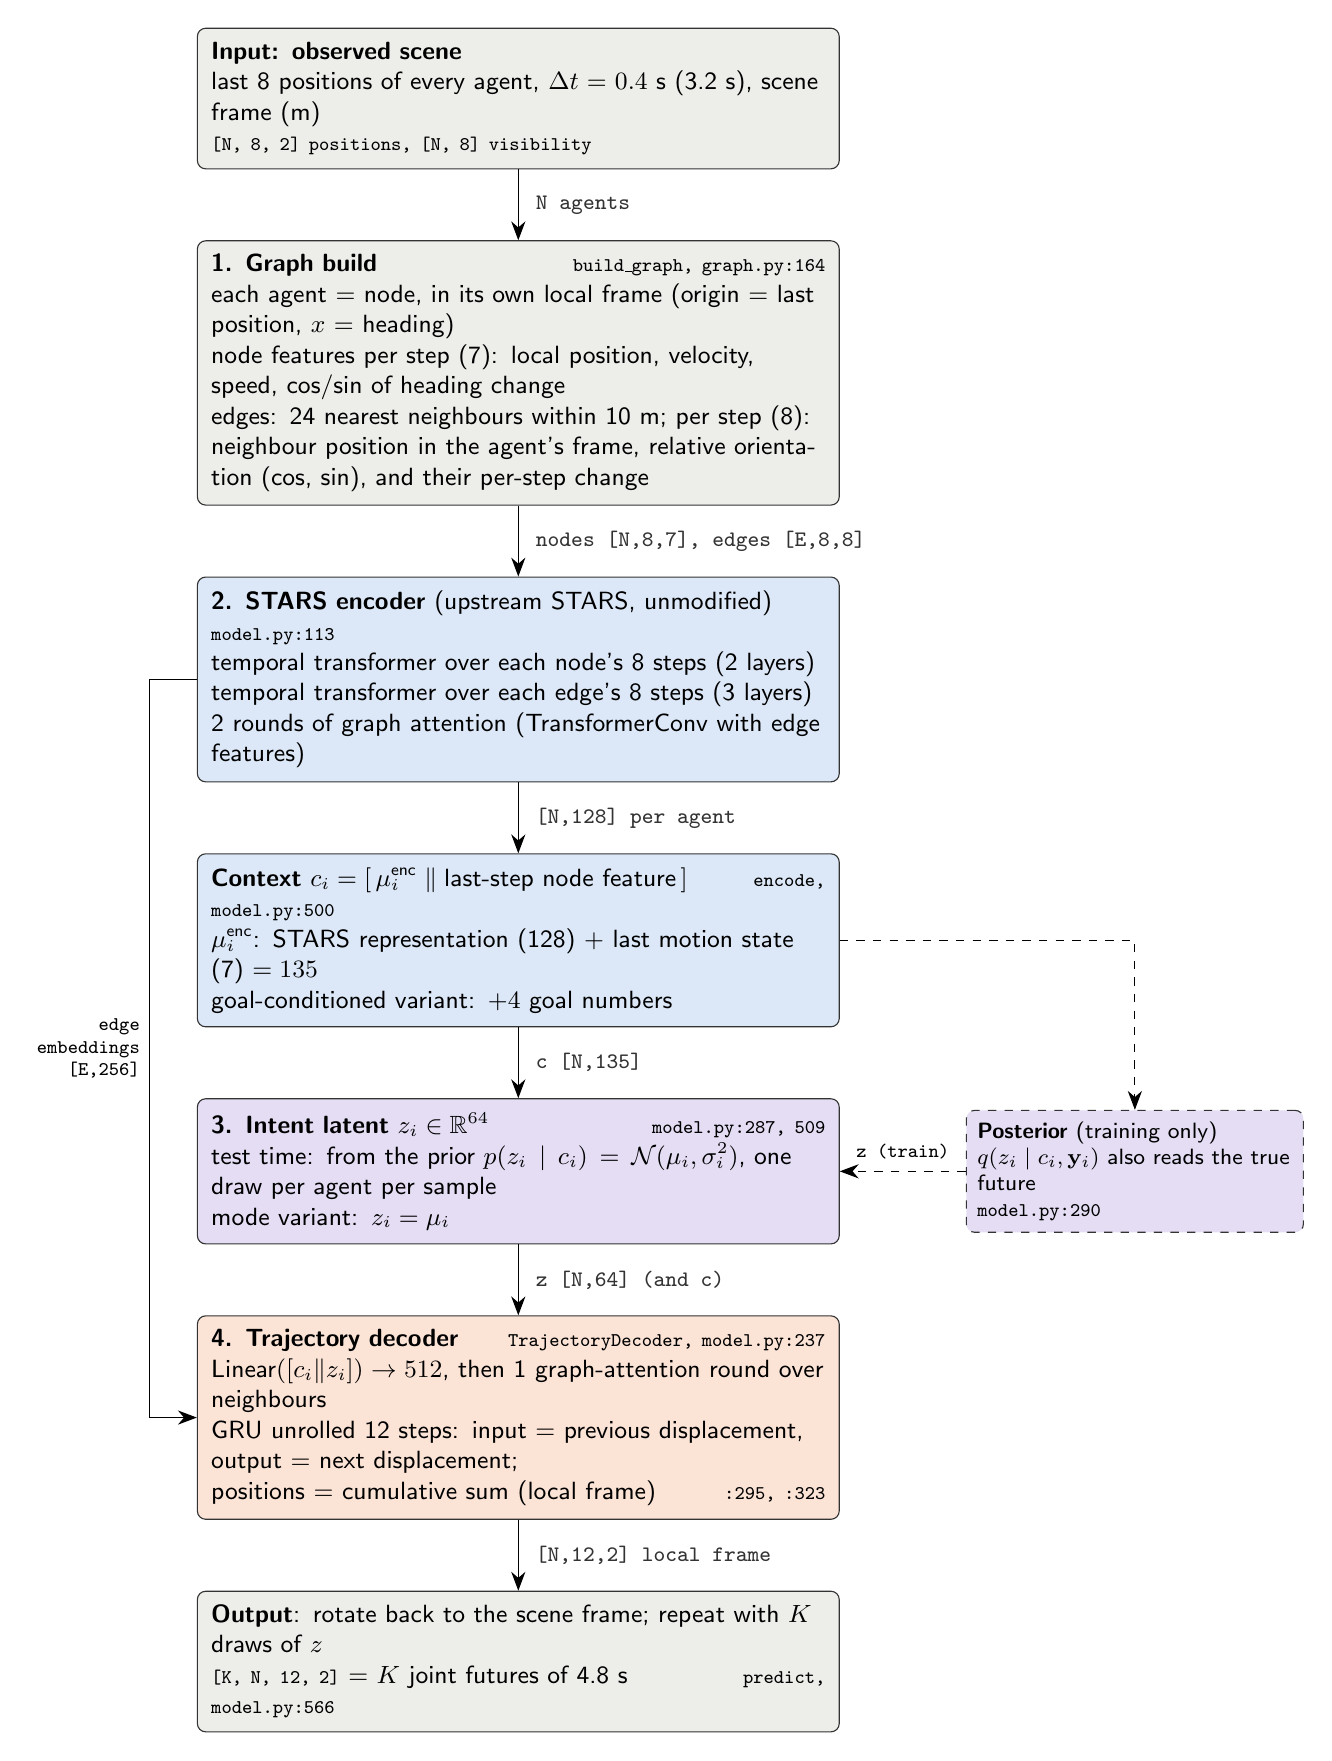
\begin{tikzpicture}[
  font=\sffamily\small, >={Stealth[length=2.4mm]}, node distance=9mm,
  blk/.style={draw=ink, rounded corners=3pt, align=left, text width=78mm, inner sep=5pt},
  side/.style={draw=ink, rounded corners=3pt, align=left, text width=40mm, inner sep=4pt, font=\sffamily\footnotesize},
  shp/.style={font=\ttfamily\footnotesize, text=ink, right=1mm, midway, anchor=west},
  ref/.style={font=\ttfamily\scriptsize, text=ink!70}]
\node[blk, fill=inp] (in) {\textbf{Input: observed scene}\\
  last 8 positions of every agent, $\Delta t=0.4$ s (3.2 s), scene frame (m)\\
  {\ttfamily\scriptsize [N, 8, 2] positions,\ [N, 8] visibility}};
\node[blk, fill=inp, below=of in] (g) {\textbf{1. Graph build} \hfill{\ttfamily\scriptsize build\_graph, graph.py:164}\\
  each agent = node, in its own local frame (origin = last position, $x$ = heading)\\
  node features per step (7): local position, velocity, speed, cos/sin of heading change\\
  edges: 24 nearest neighbours within 10 m; per step (8): neighbour position in the agent's frame, relative orientation (cos, sin), and their per-step change};
\node[blk, fill=enc, below=of g] (e) {\textbf{2. STARS encoder} (upstream STARS, unmodified) \hfill{\ttfamily\scriptsize model.py:113}\\
  temporal transformer over each node's 8 steps (2 layers)\\
  temporal transformer over each edge's 8 steps (3 layers)\\
  2 rounds of graph attention (TransformerConv with edge features)};
\node[blk, fill=enc, below=of e] (c) {\textbf{Context} $c_i=[\,\mu^{\text{enc}}_i \;\|\; \text{last-step node feature}\,]$ \hfill{\ttfamily\scriptsize encode, model.py:500}\\
  $\mu^{\text{enc}}_i$: STARS representation (128) + last motion state (7) $=135$\\
  goal-conditioned variant: $+4$ goal numbers};
\node[blk, fill=lat, below=of c] (z) {\textbf{3. Intent latent} $z_i\in\mathbb R^{64}$ \hfill{\ttfamily\scriptsize model.py:287, 509}\\
  test time: from the prior $p(z_i\mid c_i)=\mathcal N(\mu_i,\sigma_i^2)$, one draw per agent per sample\\
  mode variant: $z_i=\mu_i$};
\node[side, fill=lat, dashed, right=16mm of z] (q) {\textbf{Posterior} (training only)\\ $q(z_i\mid c_i,\mathbf y_i)$ also reads the true future\\ {\ttfamily\scriptsize model.py:290}};
\node[blk, fill=dec, below=of z] (d) {\textbf{4. Trajectory decoder} \hfill{\ttfamily\scriptsize TrajectoryDecoder, model.py:237}\\
  Linear$([c_i\|z_i])\to512$, then 1 graph-attention round over neighbours\\
  GRU unrolled 12 steps: input = previous displacement, output = next displacement;\\
  positions = cumulative sum (local frame) \hfill{\ttfamily\scriptsize :295, :323}};
\node[blk, fill=inp, below=of d] (o) {\textbf{Output}: rotate back to the scene frame; repeat with $K$ draws of $z$\\
  {\ttfamily\scriptsize [K, N, 12, 2]} = $K$ joint futures of 4.8 s \hfill{\ttfamily\scriptsize predict, model.py:566}};
\draw[->] (in) -- node[shp]{N agents} (g);
\draw[->] (g) -- node[shp]{nodes [N,8,7], edges [E,8,8]} (e);
\draw[->] (e) -- node[shp]{[N,128] per agent} (c);
\draw[->] (c) -- node[shp]{c [N,135]} (z);
\draw[->] (z) -- node[shp]{z [N,64] (and c)} (d);
\draw[->] (d) -- node[shp]{[N,12,2] local frame} (o);
\draw[->, dashed] (q) -- node[above=1pt, font=\ttfamily\scriptsize]{z (train)} (z);
\draw[->, dashed] (c.east) -| (q.north);
\draw[->] (e.west) -- ++(-6mm,0) |- node[pos=0.25, left, font=\ttfamily\scriptsize, align=right]{edge\\embeddings\\{[E,256]}} (d.west);
\end{tikzpicture}
\caption{The core STARS forecaster (CVAE), top to bottom, with tensor shapes for one scene of $N$ agents and
$E$ directed edges. ``graph.py'' $=$ \code{src/baselines/stars\_ma\_graph.py}, ``model.py'' $=$
\code{src/baselines/stars\_ma\_model.py}. The encoder is the upstream STARS \code{CombinedHGNNEncoder}
(\code{references/stars/src/models/hgnn\_combined\_v2.py:85}).}
\label{fig:core}
\end{figure}

\clearpage
\paragraph{1. Graph build} (\code{build\_graph}, \code{stars\_ma\_graph.py:164}). Every agent visible at the last
observed step becomes a node. For each node and each of the 8 observed steps, the \textbf{node feature}
(7 numbers, \code{:105}) is its position and velocity in its own local frame, its speed, and the cosine/sine
of its heading relative to its current heading. Directed \textbf{edges} connect each agent to its 24
nearest neighbours within 10 m at the last observed step (\code{:136}). Each edge carries, per step, 8
numbers (\code{:117}): the neighbour's position in the source agent's frame (2), their relative orientation
(cos, sin), and the per-step change of these four.

\paragraph{2. STARS encoder} (\code{StarsMotionEncoder}, \code{stars\_ma\_model.py:113}). A temporal transformer
summarises each node's 8-step feature sequence (2 layers) and each edge's 8-step sequence (3 layers);
two rounds of graph attention (\code{TransformerConv} with edge features) mix information between
neighbours. Output per agent: the STARS representation $\mu^{\text{enc}}_i\in\mathbb R^{128}$ (the mean
head of STARS's own VAE, \code{forward} at \code{:156}); per edge: an embedding in $\mathbb R^{256}$.

\paragraph{3. Context and intent latent.} The decoder context is
$c_i = [\mu^{\text{enc}}_i \,\|\, \text{node feature at the last step}]\in\mathbb R^{135}$
(\code{encode}, \code{:500}). A small MLP gives a Gaussian \textbf{prior} $p(z_i\mid c_i)$ over a
64-dimensional intent $z_i$ (\code{prior\_params}, \code{:287}). During training, a \textbf{posterior}
$q(z_i\mid c_i,\mathbf y_i)$ also sees the agent's true future (\code{:290}); at test time $z_i$ is drawn
from the prior (\code{sample\_latent}, \code{:509}). One $z_i$ is drawn per agent, independently.

\paragraph{4. Decoder} (\code{TrajectoryDecoder.forward}, \code{:323}). $[c_i\|z_i]$ is projected to 512
units, one \code{TransformerConv} round lets each agent attend to its neighbours' (context, intent),
and a GRU unrolls 12 steps (\code{rollout\_steps}, \code{:295}): each step takes the previous displacement
and outputs the next one; positions are the cumulative sum. Output: \shape{N, 12, 2} in each agent's
local frame. Repeating with $K$ independent draws of $z$ gives $K$ samples (\code{predict}, \code{:566}).

%======================================================================
\section{Inputs and outputs, with a worked example}
%======================================================================

\begin{tabularx}{\textwidth}{@{}l l X@{}}
\toprule
& Shape & Content \\
\midrule
\textbf{In} & \shape{N, 8, 2} & observed positions (scene frame, m), NaN where not visible \\
& \shape{N, 8} & visibility mask \\
& \shape{N, 4} (optional) & goal input: $(\Delta x,\Delta y)$ to the goal in the local frame, distance (all $/10$ m), valid flag --- goal-conditioned variant only (\code{goal\_features}, \code{:73}) \\
\midrule
\textbf{Internal} & \shape{N, 8, 7}, \shape{E, 8, 8} & node and edge features \\
& \shape{N, 128} $\to$ \shape{N, 135} & encoder representation $\to$ decoder context \\
& \shape{N, 64} & intent latent $z$ (one per agent per sample) \\
\midrule
\textbf{Out} & \shape{K, N, 12, 2} & $K$ joint futures, 12 steps of 0.4 s (scene frame, m) \\
\bottomrule
\end{tabularx}

\subsection*{Example: two people approaching each other}
Alice walks east at 1.2 m/s and is now at $(0,0)$; Bob walks west at 1.0 m/s and is now at $(6.0, 0.3)$.
\begin{itemize}
\item \textbf{Input.} Alice's 8 observed positions are $(-3.36,0),(-2.88,0),\dots,(0,0)$ (0.48 m per step);
Bob's are $(8.8,0.3),\dots,(6.0,0.3)$ (0.40 m per step). \shape{2,8,2}.
\item \textbf{Local frames.} Alice: origin $(0,0)$, heading $0$. Bob: origin $(6.0,0.3)$, heading $\pi$.
\item \textbf{Node feature, last step.} Both are at their own origin moving forward:
Alice $(0,0,\;1.2,0,\;1.2,\;1,0)$, Bob $(0,0,\;1.0,0,\;1.0,\;1,0)$ = (position, velocity, speed,
cos/sin of relative heading).
\item \textbf{Edge Bob$\to$Alice, last step.} Alice as seen from Bob, in Bob's frame: $(6.0,\,0.3)$ (6 m ahead, 0.3 m to his left), relative orientation $(\cos,\sin)=(-1,0)$ (facing each other), and per-step change
$(-0.88,\,0,\,0,\,0)$ (closing at $2.2$ m/s $\times 0.4$ s). One such 8-vector per observed step.
\item \textbf{Encoder/decoder.} Context $c\in\mathbb R^{2\times135}$; for each of the $K=20$ samples,
$z\in\mathbb R^{2\times64}$ is drawn from the prior and decoded.
\item \textbf{Output} \shape{20,2,12,2}. An illustrative sample $k$: Alice continues east and drifts
0.3--0.4 m to her left over the first 2 s; Bob drifts to his left; they pass at about 0.7 m. Another sample may
have both drifting the same way --- the per-agent latents are drawn independently, which is what the
oversampling and collision-aware variants address.
\end{itemize}

%======================================================================
\section{Variants}
%======================================================================

\begin{figure}[h!]
\centering
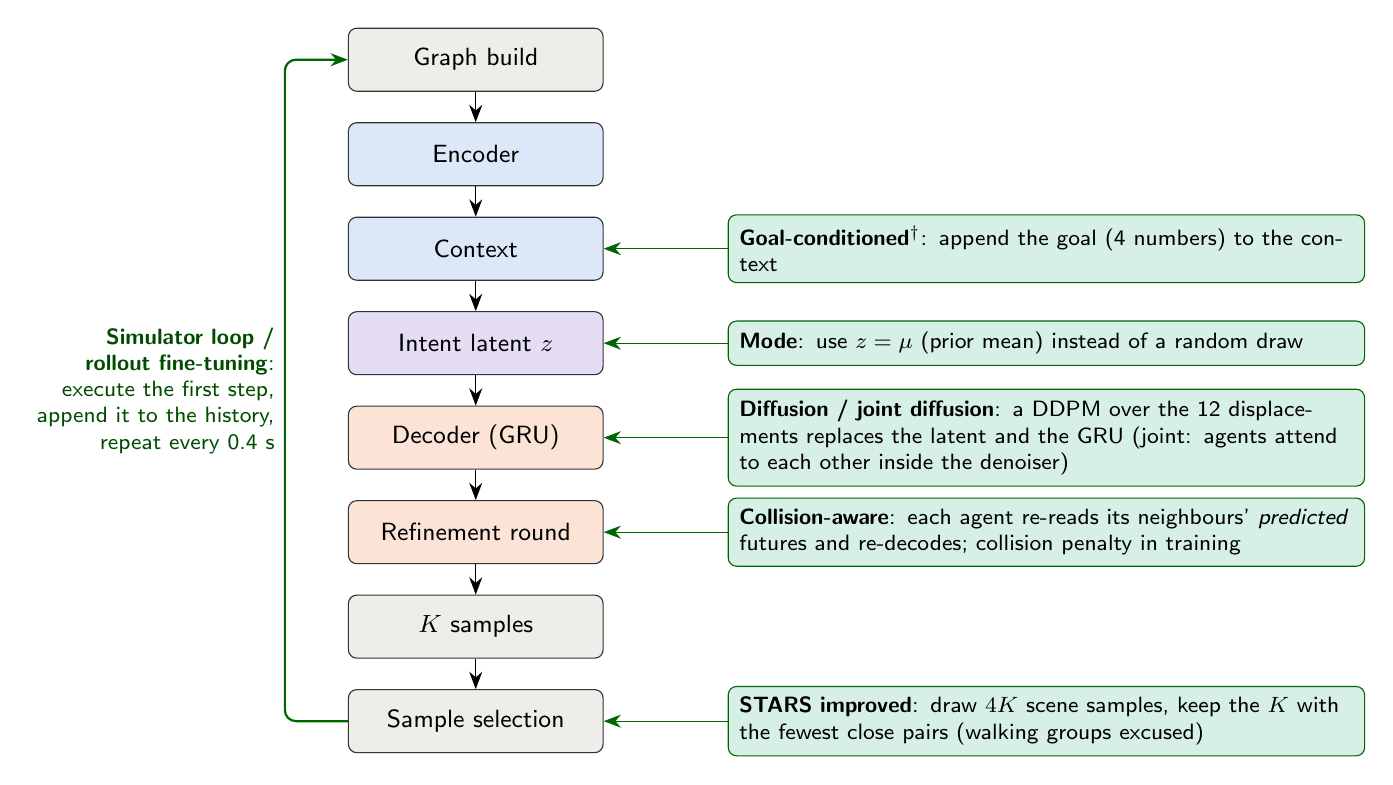
\begin{tikzpicture}[font=\sffamily\small, >={Stealth[length=2.2mm]},
  st/.style={draw=ink, rounded corners=3pt, align=center, minimum height=8mm, text width=30mm},
  vr/.style={draw=green!40!black, fill=var, rounded corners=3pt, align=left, text width=78mm, inner sep=4pt, font=\sffamily\footnotesize}]
\foreach \n/\t/\f/\y in {g/Graph build/inp/0, e/Encoder/enc/-1.2, c/Context/enc/-2.4, z/Intent latent $z$/lat/-3.6,
                          d/Decoder (GRU)/dec/-4.8, r/Refinement round/dec/-6.0, k/$K$ samples/inp/-7.2, s/Sample selection/inp/-8.4}
  \node[st, fill=\f] (\n) at (0,\y) {\t};
\foreach \a/\b in {g/e,e/c,c/z,z/d,d/r,r/k,k/s} \draw[->] (\a) -- (\b);
\node[vr, anchor=west] (vg) at (3.2,-2.4) {\textbf{Goal-conditioned}$^\dagger$: append the goal (4 numbers) to the context};
\node[vr, anchor=west] (vm) at (3.2,-3.6) {\textbf{Mode}: use $z=\mu$ (prior mean) instead of a random draw};
\node[vr, anchor=west] (vd) at (3.2,-4.8) {\textbf{Diffusion / joint diffusion}: a DDPM over the 12 displacements replaces the latent and the GRU (joint: agents attend to each other inside the denoiser)};
\node[vr, anchor=west] (vr) at (3.2,-6.0) {\textbf{Collision-aware}: each agent re-reads its neighbours' \emph{predicted} futures and re-decodes; collision penalty in training};
\node[vr, anchor=west] (vs) at (3.2,-8.4) {\textbf{STARS improved}: draw $4K$ scene samples, keep the $K$ with the fewest close pairs (walking groups excused)};
\foreach \a/\b in {vg/c,vm/z,vd/d,vr/r,vs/s} \draw[->, green!40!black] (\a.west) -- (\b.east);
\draw[->, green!40!black, thick, rounded corners] (s.west) -- ++(-8mm,0) |- node[pos=0.25, left, align=right, font=\sffamily\footnotesize, text=green!30!black]
  {\textbf{Simulator loop /}\\ \textbf{rollout fine-tuning}:\\ execute the first step,\\ append it to the history,\\ repeat every 0.4 s} (g.west);
\end{tikzpicture}
\caption{Where each variant changes the pipeline (the refinement round and the sample selection are not in the core model).
$^\dagger$ uses privileged information (the true endpoint). Rollout fine-tuning trains the whole stack through the
simulator loop on the left.}
\label{fig:variants}
\end{figure}

{\footnotesize
\begin{tabularx}{\textwidth}{@{}>{\raggedright}p{2.4cm} >{\raggedright}X >{\raggedright}p{2.5cm} >{\raggedright\arraybackslash}p{3.8cm}@{}}
\toprule
Variant & What changes & Code & Checkpoint \\
\midrule
STARS (STEPS-only) & core model, STEPS only; latent 32, kNN 16 & config steps.yaml & \cp{cvae_kl01_finetune} \\
STARS previous (pooled) & core model; 6 datasets (incl.\ ETH/UCY) & config all.yaml & \cp{cvae_all_lr3e-4_seed42} \\
STARS improved & 7 datasets (+ATC); keep the $K$ least-colliding of $4K$ scene samples & model.py:573, :592 & \cp{si_final_base_s2} with \cp{oversample: 4} \\
Mode & $z=\mu$ of the prior: one deterministic future & model.py:514 & any CVAE checkpoint \\
Collision-aware & refinement round over neighbours' \emph{predicted} futures; collision hinge in training; KL 0.15 & model.py:273--282, :337--344; train:405 & \cp{si_final_social_s42} \\
Goal-conditioned$^\dagger$ & goal features appended to the context & model.py:73, :505 & \cp{cvae_noethucy_goal} \\
Diffusion (per-agent / joint) & DDPM over displacements replaces latent and GRU; joint = social layers inside the denoiser & model.py:348 & STEPS-trained runs \\
Rollout fine-tuned & fine-tuned on its own closed-loop rollouts & model.py:621; train:458 & \cp{rft_base_noatc} \\
\bottomrule
\end{tabularx}}

\noindent{\footnotesize Configs are in \code{configs/stars\_ma/}; ``model.py'' $=$ \code{stars\_ma\_model.py}; ``train:'' $=$
\code{train\_stars\_ma.py}. Checkpoints are in \cp{experiments/stars_ma/runs/<name>/checkpoints/best.pt}.
In progress on branch \code{ethucy-protocol}: pretraining on STEPS, PTDPES, Madras and Grand Central only
(\code{ep\_pre4\_s*}) and leave-one-scene-out fine-tuning on ETH/UCY (\code{ep\_loso\_*}).}

\subsection{STARS improved: least-colliding sample selection (inference only)}
Draw $M\cdot K$ joint samples ($M=4$), count for each sample the agent pairs that come within 0.4 m at
some future step, \emph{excluding} pairs that look like a walking group in the observation (within 1 m
and velocities within 0.3 m/s at the last observed step, \code{observed\_groups} :582), and keep the $K$
samples with the fewest such pairs (\code{select\_scene\_samples} :592). Only the model's own samples and
the observed history are used. In the simulator the same idea is applied to whole rollouts
(\code{Stars.with\_oversample}, \code{sim.py:174}).

\subsection{Collision-aware: refinement round}
After the first decoding pass, each agent re-reads its neighbours through a second
\code{TransformerConv} whose edge features are built from the neighbours' \emph{predicted} futures
(\code{future\_edges} :309): the neighbour's predicted position relative to the agent at each of the 12
steps (in the agent's frame), its per-step change, and the closest predicted approach, \shape{E, 4P+1}. The
hidden state is updated and the GRU re-decodes (:337--344). These are the model's own predictions, so this
runs identically at test time. The collision hinge (Appendix~\ref{app:loss}) is used only in training.

\subsection{Mode}
Instead of $z=\mu+\sigma\epsilon$, use $z=\mu$. This gives the single most likely future and is the fair
comparison with deterministic baselines such as constant velocity.

\subsection{Goal-conditioned$^\dagger$}
The context gets four extra numbers: the goal relative to the agent (local frame, $/10$ m), its distance
and a valid flag. In the benchmarks the goal is the track's last recorded position (an oracle), so these
rows are marked as privileged.

\subsection{Diffusion decoders}
The latent and GRU are replaced by a DDPM over the 12 per-step displacements minus constant-velocity
steps, scaled by 0.1 m (\code{DiffusionDecoder} :348; MID-style). The per-agent version denoises each agent
independently given its socially mixed hidden state; the joint version (MotionDiffuser-style) puts social
\code{TransformerConv} layers inside the denoiser so all agents of a sample are denoised together. Sampling
is deterministic DDIM.

%======================================================================
\section{Closed loop: STARS as a crowd simulator}
%======================================================================
\begin{figure}[h!]
\centering
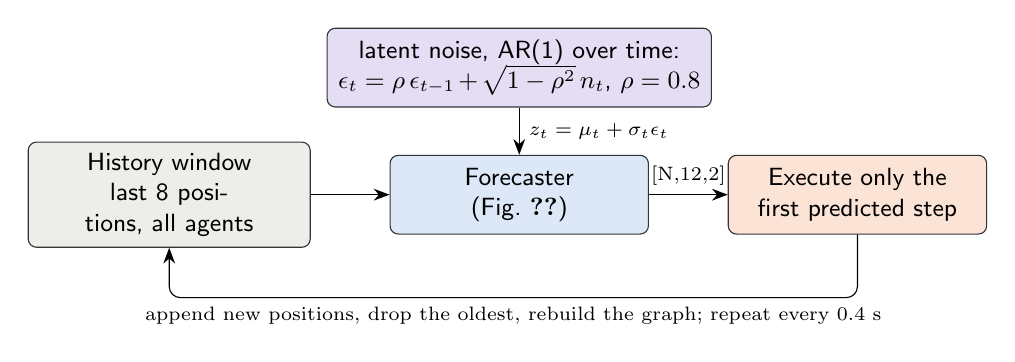
\begin{tikzpicture}[font=\sffamily\small, >={Stealth[length=2mm]},
  blk/.style={draw=ink, rounded corners=3pt, align=center, minimum height=10mm, inner sep=4pt}]
\node[blk, fill=inp, text width=33mm] (w) {History window\\ last 8 positions, all agents};
\node[blk, fill=enc, right=10mm of w, text width=30mm] (f) {Forecaster\\ (Fig.~\ref{fig:core})};
\node[blk, fill=lat, above=6mm of f, text width=46mm] (n) {latent noise, AR(1) over time:\\ $\epsilon_t=\rho\,\epsilon_{t-1}+\sqrt{1-\rho^2}\,n_t$, $\rho=0.8$};
\node[blk, fill=dec, right=10mm of f, text width=30mm] (x) {Execute only the\\ first predicted step};
\draw[->] (w) -- (f);
\draw[->] (n) -- node[right, font=\scriptsize]{$z_t=\mu_t+\sigma_t\epsilon_t$} (f);
\draw[->] (f) -- node[above, font=\scriptsize]{[N,12,2]} (x);
\draw[->, rounded corners] (x.south) -- ++(0,-8mm) -| node[pos=0.25, below, font=\scriptsize]{append new positions, drop the oldest, rebuild the graph; repeat every 0.4 s} (w.south);
\end{tikzpicture}
\caption{Closed loop (\code{Stars.\_rollout}, \code{src/simplenavsim/realism/sim.py:200};
the training-time copy is \code{closed\_loop\_rollout}, \code{stars\_ma\_model.py:621}). The AR(1) noise keeps
each agent's intent consistent over time while letting it change slowly.}
\end{figure}

\noindent Rollout fine-tuning trains exactly this loop: it unrolls 4 to 12 steps of it on training
windows, with gradients through the executed positions into later steps' graphs, and penalises the
distance to the true positions (Appendix~\ref{app:loss}).

%======================================================================
\appendix
\section{Loss functions}\label{app:loss}
%======================================================================
All position losses are computed in each agent's local frame unless noted; $\mathcal V=\{(i,t): m_{i,t}=1\}$
is the set of supervised (agent, future step) pairs.

\paragraph{CVAE prior and posterior.} $p(z_i\mid c_i)=\mathcal N(\mu^p_i,\operatorname{diag}\sigma^{p\,2}_i)$,
$q(z_i\mid c_i,\mathbf y_i)=\mathcal N(\mu^q_i,\operatorname{diag}\sigma^{q\,2}_i)$, where the posterior also reads an MLP
encoding of the masked true future. Training uses $z_i=\mu^q_i+\sigma^q_i\odot\epsilon$, $\epsilon\sim\mathcal N(0,I)$
(agents with no supervised future use the prior). (\code{training\_forward}, \code{stars\_ma\_model.py:530}.)

\paragraph{Forecast (reconstruction) loss} (\code{\_masked\_distance}, \code{train\_stars\_ma.py:399}):
\[
\mathcal L_{\text{fc}}=\frac{1}{|\mathcal V|}\sum_{(i,t)\in\mathcal V}\big\|\hat{\mathbf y}_{i,t}(z^q_i)-\mathbf y_{i,t}\big\|_2 .
\]

\paragraph{KL term} (\code{stars\_ma\_model.py:554}), averaged over agents with a supervised future:
\[
\mathcal L_{\text{KL}}=\frac{1}{N_f}\sum_i \tfrac12\sum_{d=1}^{64}\Big[\log\tfrac{\sigma^{p\,2}_{i,d}}{\sigma^{q\,2}_{i,d}}
+\frac{\sigma^{q\,2}_{i,d}+(\mu^q_{i,d}-\mu^p_{i,d})^2}{\sigma^{p\,2}_{i,d}}-1\Big],
\]
weighted by $\beta$ ($0.0799$; $0.15$ for collision-aware), linearly warmed up over the first 10 epochs
(\code{train\_stars\_ma.py:875}).
(\code{train\_stars\_ma.py:875}).

\paragraph{Collision hinge} (collision-aware only; \code{collision\_loss}, \code{train\_stars\_ma.py:405}). On a
prior sample decoded with its latent detached (so it trains the decoder but cannot widen the prior),
for every graph edge $(i,j)$ and future step $t$ where both are supervised:
\[
\mathcal L_{\text{col}}=\frac{1}{|\mathcal V|}\sum_{(i,j)\in E}\sum_t m_{i,t}m_{j,t}\,
\operatorname{ReLU}\!\big(r_{ij}-\|\hat{\mathbf p}_{i,t}-\hat{\mathbf p}_{j,t}\|\big),\qquad
r_{ij}=\min\!\big(0.4\text{ m},\ \min_t\|\mathbf y_{i,t}-\mathbf y_{j,t}\|\big),
\]
with $\hat{\mathbf p}$ in the scene frame. Pairs that really walk closer than 0.4 m (groups) are only pushed
to their true closest distance. Weight $\lambda_{\text{col}}=10$.

\paragraph{Best-of-many} (tried, not in a final model; \code{train\_stars\_ma.py:448}). With $S$ prior samples,
\[\mathcal L_{\text{bom}}=\frac{1}{N_f}\sum_i\min_{s\le S}\operatorname{ADE}_i\big(\hat{\mathbf y}^{(s)}_i\big).\]

\paragraph{Rollout fine-tuning} (\code{train\_stars\_ma.py:458}). Starting from a trained checkpoint, unroll
the closed loop for $L$ steps with prior latents and AR(1) noise ($\rho=0.8$), giving executed scene-frame
positions $\tilde{\mathbf p}_{i,1..L}$, and add
\[
\mathcal L_{\text{rft}}=\frac{1}{|\mathcal V_L|}\sum_{(i,t)\in\mathcal V_L,\,t\le L}\big\|\tilde{\mathbf p}_{i,t}-\mathbf y_{i,t}\big\|_2 ,
\]
with a curriculum $L=4\to12$ over 3 epochs. Gradients flow through all executed positions (no truncation).
An optional progress term $\lambda_{\text{prog}}\big|\,\|\tilde{\mathbf p}_{i,t}-\mathbf x_{i,T}\|-\|\mathbf y_{i,t}-\mathbf x_{i,T}\|\,\big|$
exists; the selected model uses $\lambda_{\text{prog}}=0$.

\paragraph{Total loss} (\code{train\_stars\_ma.py:478}):
\[
\mathcal L=w_{\text{ol}}\big(\mathcal L_{\text{fc}}+\beta\,\mathcal L_{\text{KL}}\big)
+w_{\text{rft}}\,\mathcal L_{\text{rft}}+\lambda_{\text{col}}\,\mathcal L_{\text{col}}+\lambda_{\text{bom}}\,\mathcal L_{\text{bom}},
\]
with $w_{\text{ol}}=1$ always; $w_{\text{rft}}=1$ only when fine-tuning; $\lambda_{\text{col}}=10$ only for
collision-aware; $\lambda_{\text{bom}}=0$ in all final models.

\paragraph{Diffusion decoders} (\code{DiffusionDecoder.loss}, \code{stars\_ma\_model.py:425}). Target
$\mathbf x_0=(\Delta\mathbf y_{i,t}-\mathbf v_i\Delta t)/0.1$ (displacements minus constant velocity), cosine
schedule $\bar\alpha_t=f(t)/f(0)$, $f(t)=\cos^2\!\big(\tfrac{t/T_d+0.008}{1.008}\tfrac\pi2\big)$, $T_d=100$:
\[
\mathbf x_\tau=\sqrt{\bar\alpha_\tau}\,\mathbf x_0+\sqrt{1-\bar\alpha_\tau}\,\epsilon,\qquad
\mathcal L_{\text{diff}}=\frac{\sum m\,\|\epsilon_\theta(\mathbf x_\tau,\tau,h_i)-\epsilon\|^2}{\sum m}.
\]
The joint version draws one noise level $\tau$ per scene. Sampling: deterministic DDIM.

\paragraph{Least-colliding selection} (inference). For sample $s$ of a scene,
\[C(s)=\sum_{\substack{i<j\\ (i,j)\notin\text{groups}}}\mathbf 1\Big[\min_t\big\|\hat{\mathbf p}^{(s)}_{i,t}-\hat{\mathbf p}^{(s)}_{j,t}\big\|<0.4\text{ m}\Big];\]
keep the $K$ samples with the smallest $C$ out of $4K$.

%======================================================================
\section{Hyperparameters of the main checkpoints}
%======================================================================
\begin{tabularx}{\textwidth}{@{}l l X@{}}
\toprule
Component & Setting & Value \\
\midrule
Graph & neighbours / radius & 24 / 10 m (STEPS-only model: 16) \\
Encoder & hidden / representation & 256 / 128 \\
& node / edge temporal transformer layers & 2 / 3, 4 heads \\
& message-passing rounds & 2 (TransformerConv) \\
& dropout & 0.0905 \\
Decoder & hidden / intent latent & 512 / 64 (STEPS-only: 32) \\
& social rounds / refinement rounds & 1 / 0 (collision-aware: 1) \\
& dropout & 0.0633 \\
Training & optimiser, LR & AdamW, $3\times10^{-4}$, warm-up + cosine \\
& weight decay, grad clip & 0.00217, 1.0 \\
& epochs, selection & 60, best validation best-of-20 ADE (macro over datasets) \\
& KL weight & 0.0799 (collision-aware: 0.15), 10-epoch warm-up \\
Rollout fine-tuning & LR, batches & $5\times10^{-5}$, 300 batches of 2048 agents per epoch \\
& rollout length & 4 $\to$ 12 steps over 3 epochs; 12 epochs, kept epoch 6 (best closed-loop validation ADE) \\
& data & 6 datasets without ATC (\cp{configs/stars_ma/rft_no_atc.yaml}) \\
Simulator & latent noise correlation & $\rho=0.8$ \\
\bottomrule
\end{tabularx}

%======================================================================
\section{Evaluation metrics (short definitions)}
%======================================================================
\begin{itemize}
\item \textbf{Per-agent best-of-$K$ ADE/FDE} (minADE$_{20}$): for each agent, the smallest average / final
displacement error over its $K$ samples; each agent chooses its own sample.
\item \textbf{Scene-level best-of-$K$} (joint): one sample index for all agents of a window (the one with the
lowest summed error), then average.
\item \textbf{Single-sample ADE}: error of a random sample (averaged over the $K$); \textbf{mode ADE}: error of
the $z=\mu$ prediction.
\item \textbf{Close-contact rate}: share of agents within 0.2 m / 0.4 m of another agent at some predicted
step, ignoring observed walking-group pairs; compared with the same rate in the real futures.
\item \textbf{Realism W1}: Wasserstein-1 distance between predicted and real per-step distributions of speed,
acceleration, turning rate and nearest-neighbour distance.
\item \textbf{Closed loop}: the same metrics on simulated trajectories (one rollout), plus ADE split into
near-straight and non-linear agents (mean distance from the start--end chord $>0.2$ m).
\end{itemize}

%======================================================================
\section{Code index}
%======================================================================
\begin{tabularx}{\textwidth}{@{}l l X@{}}
\toprule
File & Line & What \\
\midrule
\code{src/baselines/stars\_ma\_graph.py} & 105 & node features \shape{N,T,7} and local frames \\
& 117 & edge features \shape{E,T,8} \\
& 136 & kNN / radius edges \\
& 164 & \code{build\_graph} \\
& 196, 201 & \code{to\_local}, \code{to\_scene} \\
\code{src/baselines/stars\_ma\_model.py} & 42, 52 & encoder and decoder recipes (all options and defaults) \\
& 73 & goal features \\
& 113 & \code{StarsMotionEncoder} (wraps upstream STARS encoder) \\
& 237 & \code{TrajectoryDecoder}; prior :287, posterior :290, GRU :295, refinement :309/:337 \\
& 348 & \code{DiffusionDecoder}; loss :425, sampling :446 \\
& 472 & \code{StarsMultiAgentForecaster}; encode :500, sample\_latent :509, decode :518 \\
& 530 & \code{training\_forward} (posterior, KL, prior samples) \\
& 566 & \code{predict} (incl.\ oversampling :573) \\
& 582, 592 & observed groups, least-colliding selection \\
& 621 & \code{closed\_loop\_rollout} (used by rollout fine-tuning) \\
\code{src/baselines/train\_stars\_ma.py} & 81 & default training recipe \\
& 186--225 & command-line flags (KL, refine, collision, best-of-many, rollout fine-tuning) \\
& 399, 405 & masked distance, collision hinge \\
& 425--482 & \code{forecast\_loss}: all loss terms and their sum \\
\code{src/simplenavsim/realism/sim.py} & 27, 40 & simulator checkpoint names, oversampling \\
& 153--200 & \code{Stars} closed-loop wrapper (\code{\_rollout} :200) \\
\code{runs/stars\_rollout\_ft/rft.sh} & --- & reusable rollout fine-tuning of any checkpoint \\
\code{references/stars/src/models/hgnn\_combined\_v2.py} & 85 & upstream STARS \code{CombinedHGNNEncoder} \\
\bottomrule
\end{tabularx}

\medskip\noindent{\footnotesize The deterministic (mode) option in the closed-loop simulator,
\code{Stars(mode=True)}, is on branch \code{stars-improve}; on this branch the mode is available through
\code{sample\_latent(mean=True)}.}

\end{document}
